\documentclass[aspectratio=169,11pt]{beamer}
\def\courseweek{5}
% Shared style for the Introduction to Information Geometry lecture slides.
% Compile the lecture .tex files from this directory.
\providecommand{\courseweek}{1}
\usepackage[T1]{fontenc}
\usepackage[utf8]{inputenc}
\usepackage[sc]{mathpazo}
\renewcommand{\sfdefault}{lmss}
\renewcommand{\ttdefault}{lmtt}
\usepackage{amsmath,amssymb,mathtools}
\usepackage{tikz}
\usetikzlibrary{arrows.meta,calc,positioning}
\usepackage{pgfplots}
\pgfplotsset{compat=1.18}
\usepackage{booktabs}

\definecolor{courseink}{HTML}{173749}
\definecolor{coursemuted}{HTML}{526674}
\definecolor{courseteal}{HTML}{0E7287}
\definecolor{coursecopper}{HTML}{B66B43}
\definecolor{courseline}{HTML}{D4E0E3}
\definecolor{coursepale}{HTML}{EFF5F5}

\setbeamercolor{normal text}{fg=courseink,bg=white}
\setbeamercolor{structure}{fg=courseteal}
\setbeamercolor{frametitle}{fg=courseink,bg=white}
\setbeamercolor{title}{fg=courseink}
\setbeamercolor{subtitle}{fg=coursemuted}
\setbeamercolor{block title}{fg=courseink,bg=white}
\setbeamercolor{block body}{fg=courseink,bg=white}
\setbeamercolor{alerted text}{fg=coursecopper}
\setbeamerfont{title}{family=\rmfamily,series=\bfseries,size=\fontsize{32}{37}}
\setbeamerfont{frametitle}{family=\rmfamily,series=\bfseries,size=\fontsize{26}{31}}
\setbeamerfont{normal text}{size=\fontsize{18}{22}}
\setbeamerfont{subtitle}{size=\fontsize{17}{21}}
\setbeamersize{text margin left=0.78cm,text margin right=0.78cm}
\setbeamertemplate{navigation symbols}{}
\setbeamertemplate{itemize items}[circle]
\setbeamertemplate{enumerate items}[default]
\setbeamertemplate{blocks}[default]
\setlength{\parskip}{0.22em}
\setbeamertemplate{footline}{%
  \leavevmode\hbox to \paperwidth{\hspace{.78cm}%
  {\color{coursemuted}\fontsize{8.5}{10}\selectfont Introduction to Information Geometry \hspace{.32cm} / \hspace{.32cm} Week \courseweek}%
  \hfill{\color{coursemuted}\fontsize{8.5}{10}\selectfont \insertframenumber\hspace{.17cm}/\hspace{.17cm}\inserttotalframenumber}\hspace{.78cm}}%
  \vskip.17cm
}
\setbeamertemplate{frametitle}{%
  \vspace{.13cm}
  \insertframetitle\par
  \vspace{.08cm}
}
\setbeamertemplate{title page}{%
  \vspace*{1.00cm}
  {\color{courseteal}\fontsize{10}{13}\selectfont\bfseries
  INTRODUCTION TO INFORMATION GEOMETRY\par}
  \vspace{.40cm}
  {\usebeamerfont{title}\usebeamercolor[fg]{title}\inserttitle\par}
  \vspace{.22cm}
  {\usebeamerfont{subtitle}\usebeamercolor[fg]{subtitle}\insertsubtitle\par}
  \vfill
  {\color{coursemuted}\fontsize{13}{16}\selectfont Christopher Lee\par}
  \vspace{.34cm}
}

\pgfplotsset{
  courseplot/.style={
    width=11.05cm,
    height=5.15cm,
    axis line style={coursemuted!75},
    tick style={coursemuted!65},
    ticklabel style={font=\scriptsize,color=coursemuted},
    label style={font=\normalsize,color=courseink},
    grid=major,
    major grid style={courseline!70,line width=.4pt},
    line width=1.45pt,
    legend style={font=\small,draw=none,fill=none,at={(.98,.03)},anchor=south east},
    clip=true
  }
}

\newcommand{\highlightmath}[1]{{\color{courseteal}#1}}
\newcommand{\thinrule}{\par\vspace{.25cm}{\color{courseline}\rule{\linewidth}{.8pt}}\par}

% A one-dimensional state space.  x=0 and x=1 are placed at 0 and 9 units.
\newcommand{\stateinterval}[1]{%
 \begin{tikzpicture}[x=1cm,y=1cm]
   \draw[courseink,line width=1.25pt] (0,0)--(9,0);
   \foreach \pos/\lab in {0/0,9/1} {
     \fill[courseink] (\pos,0) circle(2.7pt);
     \node[below=9pt,text=coursemuted] at (\pos,0) {\(\lab\)};
   }
   #1
 \end{tikzpicture}%
}

% Paired pages are separate frames in the PDF, with matching titles.
% Supply the whole frame body for each version; the instructor may edit them
% independently without changing overlay logic.
\newcommand{\coursepair}[3]{%
  \begin{frame}{#1}#2\end{frame}%
  \begin{frame}{#1}#3\end{frame}%
}

% Equilateral representation of the categorical simplex, in barycentric
% coordinates with vertices A=(0,0), B=(1,0), C=(1/2,sqrt(3)/2).
\newcommand{\coursesimplex}[1]{%
 \begin{tikzpicture}[scale=4.9]
  \fill[coursepale] (0,0)--(1,0)--(.5,.8660254)--cycle;
  \draw[courseink,line width=.65pt] (0,0)--(1,0)--(.5,.8660254)--cycle;
  \node[below left,font=\small] at (0,0) {A};
  \node[below right,font=\small] at (1,0) {B};
  \node[above,font=\small] at (.5,.8660254) {C};
  #1
 \end{tikzpicture}%
}

\title{Log-Odds and Exponential Updating}
\subtitle{Week 5 \(\cdot\) Lecture 2}
\date{}
\begin{document}
\begin{frame}[plain]\titlepage\end{frame}

\begin{frame}{Odds and log-odds}
For a Bernoulli law \((x,1-x)\), the odds of A against B are
\[
\frac{x}{1-x}.
\]
\vspace{.4cm}
The log-odds coordinate is
\[
\highlightmath{y=\ln\frac{x}{1-x}},\qquad 0<x<1.
\]
\vspace{.38cm}
As \(x\) ranges through the interval, \(y\) ranges through \(\mathbb R\).
\end{frame}

\begin{frame}{From the log-odds line to the interval}
Solving for \(x\) gives
\[
\highlightmath{x=\frac{e^y}{1+e^y}}.
\]
\vspace{-.16cm}
\begin{center}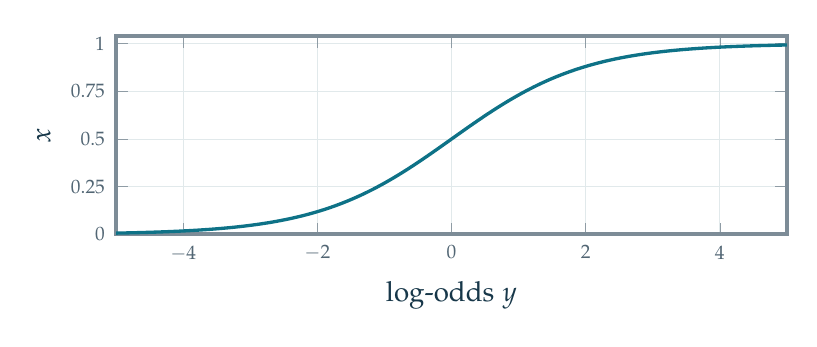
\begin{tikzpicture}
\begin{axis}[courseplot,width=10.1cm,height=4.10cm,xmin=-5,xmax=5,
 ymin=0,ymax=1.04,xlabel={log-odds $y$},ylabel={$x$},
 xtick={-4,-2,0,2,4},ytick={0,.25,.5,.75,1}]
\addplot[courseteal,very thick,domain=-5:5,samples=160]{1/(1+exp(-x))};
\end{axis}\end{tikzpicture}\end{center}
\end{frame}

\coursepair{A particular log-odds value}{
Find the log-odds for a probability of \(x=0.2\):
\vspace{.55cm}
\[
y=\ln\frac{0.2}{0.8}=\;?.
\]
\vspace{.38cm}
Is this state above or below the equal mixture \(x=\frac12\)?
}{
Find the log-odds for a probability of \(x=0.2\):
\vspace{.55cm}
\[
\highlightmath{y=\ln\frac14=-\ln4}.
\]
\vspace{.38cm}
It is negative, corresponding to \(x<\frac12\).
}

\begin{frame}{The replicator equation in log-odds}
Differentiate \(y=\ln x-\ln(1-x)\):
\[
\frac{dy}{dx}=\frac{1}{x(1-x)}.
\]
\vspace{.45cm}
Since \(x'=x(1-x)(f_A-f_B)\), the chain rule gives
\[
\highlightmath{y'=f_A-f_B}.
\]
\vspace{.35cm}
The log-odds rate is exactly the relative fitness advantage.
\end{frame}

\begin{frame}{Constant advantage becomes linear motion}
If \(f_A-f_B=k\) is constant, then
\[
y'=k,\qquad\highlightmath{y(t)=y_0+kt}.
\]
\vspace{.5cm}
Converting back to probability gives
\[
x(t)=\frac{e^{y_0+kt}}{1+e^{y_0+kt}}.
\]
\vspace{.40cm}
This is the logistic solution from Week 1.
\end{frame}

\begin{frame}{Exponential updating for many types}
With constant fitness values \(f_1,\ldots,f_n\),
\[
\highlightmath{p_i(t)=\frac{p_i(0)e^{f_it}}{Z(t)}}.
\]
\vspace{.42cm}
The normalizing factor is
\[
\highlightmath{Z(t)=\sum_j p_j(0)e^{f_jt}}.
\]
\vspace{.4cm}
The exponential weights remain positive and sum to one after normalization.
\end{frame}

\coursepair{An exponential update with three types}{
Let \(P(0)=(.2,.3,.5)\), \(f=(1,0,-1)\), and \(t=\ln2\).
\vspace{.36cm}
Compute the unnormalized weights and the updated law:
\[
(p_i(0)e^{f_it})_i=(\;?,\;?,\;?),
\qquad P(t)=\;?.
\]
}{
Let \(P(0)=(.2,.3,.5)\), \(f=(1,0,-1)\), and \(t=\ln2\).
\vspace{.36cm}
The weights are \((.4,.3,.25)\), with \(Z=.95\).
\[
\highlightmath{P(t)=(\tfrac8{19},\tfrac6{19},\tfrac5{19})}.
\]
}

\begin{frame}{The log-normalizer describes mean fitness}
Differentiate \(Z(t)\):
\[
\highlightmath{\frac{d}{dt}\ln Z(t)=\sum_i p_i(t)f_i=\bar f(t)}.
\]
\vspace{.52cm}
Differentiating again gives
\[
\highlightmath{\frac{d^2}{dt^2}\ln Z(t)
=\sum_i p_i(t)(f_i-\bar f(t))^2}.
\]
\vspace{.35cm}
The second derivative is the fitness variance.
\end{frame}

\coursepair{Derivatives of a log-normalizer}{
At \(t=0\), let \(P=(.2,.3,.5)\) and \(f=(1,0,-1)\).
\vspace{.38cm}
Compute \(\bar f\) and \(\operatorname{Var}_P(f)\).
\vspace{.35cm}
\[
\bar f=\;?,\qquad \operatorname{Var}_P(f)=\;?.
\]
}{
At \(t=0\), let \(P=(.2,.3,.5)\) and \(f=(1,0,-1)\).
\vspace{.38cm}
\[
\bar f=.2-.5=\highlightmath{-.3}.
\]
\vspace{.35cm}
\[
\operatorname{Var}_P(f)=.7-(-.3)^2=\highlightmath{.61}.
\]
}

\begin{frame}{A mean constraint produces exponential weights}
To maximize entropy subject to a fixed expectation of values \(z_i\),
use a Lagrange multiplier \(\lambda\).
\vspace{.41cm}
The resulting probabilities have the form
\[
\highlightmath{p_i=\frac{e^{\lambda z_i}}{\sum_j e^{\lambda z_j}}}.
\]
\vspace{.45cm}
The multiplier is chosen so the required mean is attained.
\end{frame}

\begin{frame}{Entropy need not move monotonically}
For a two-type constant-advantage system with \(k>0\),
\(x(t)\) increases toward 1.
\vspace{.43cm}
Starting from \(x(0)=.2\), the binary entropy first increases
until \(x=\frac12\), then decreases.
\vspace{.4cm}
Entropy concerns the current distribution of outcomes.
The replicator field determines the direction of its change.
\end{frame}

\begin{frame}{The transition to relative entropy}
The log-probability \(\ln p_i\) appears in surprisal, entropy,
log-odds, and exponential updating.
\vspace{.5cm}
In Week 6, we compare two entire probability laws using
expected differences of their log-probabilities.
\end{frame}
\end{document}
